\section{Durchführung}
\label{sec:Durchführung}

\begin{figure}[H]
  \centering
  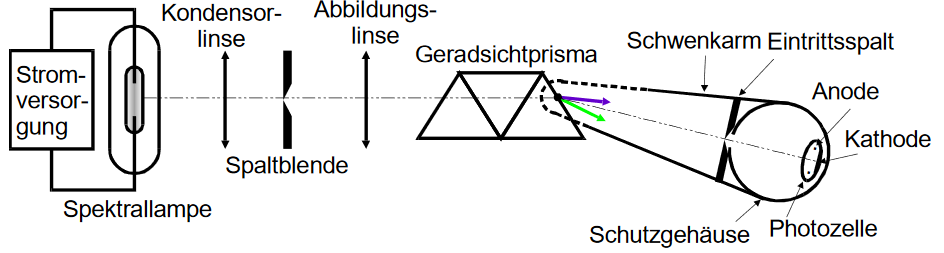
\includegraphics[height=4cm]{Versuchsaufbau.PNG}
  \caption{Aufbau zur Modifikation des Lichtweges. \cite{sample}}
  \label{fig:Aufbau}
\end{figure}

Der Versuch wird entsprechend Abbildung \ref{fig:Aufbau} aufgebaut. Zudem wird an
die Photozelle eine Spannung angelegt, welche mit einem ebenfalls angeschlossenen
Digitalvoltmeter gemessen werden kann (Abbildung \ref{fig:kathode}). Hinzu kommt noch
ein Picoamperemeter, welches zur Messung des Photostroms dient.
Anschließend werden die optischen Elemente des Aufbaus genau justiert, sodass
an der Photozelle möglichst scharfe leuchtende Streifen der einzelnen Farben zu erkennen sind.
Dabei gelingt es nicht, die Farben rot und gelb eindeutig sichtbar zu machen.
Der rote Streifen ist nur leicht sichtbar, wohingegen der eigentlich gelbe Streifen
in ein leichtes orange übergeht. Da dieses Problem sich jedoch auch nach mehreren
Lösungsversuchen nicht vollkommen beheben lässt, wird der Versuch mit der best möglichen
zu erreichenden Konfiguration durchgeführt.
Als erstes wird die Apparatur so ausgerichtet, dass das orangene (gelbe) Licht in
das Loch der Photozelle fällt. Sogleich wird eine Spannung zwischen Anode und Kathode angelegt.
In Abhängigkeit von dieser Spannung wird nun der Photostrom mithilfe des Picoamperemeters gemessen.
Dies wird für mehrere Spannungsbeträge zwischen -20V und 20V durchgeführt. Anschließend wird diese
Messung auch für alle anderen vorhandenen Farben (rot, grün, violett, ultraviolett) wiederholt.
Dabei wird sich jedoch nur auf den Spannungsbereich konzentriert, in dem sich der Photostrom am
stärksten ändert. Um das Einfallen der entsprechenden Farben in das Loch der Photozelle zu realisieren,
muss die Apparatur wiederum entsprechend ausgerichtet werden.
